\documentclass[a4paper,12pt]{report}

% ============================================================
% PACKAGES
% ============================================================
\usepackage[utf8]{inputenc}
\usepackage[T1]{fontenc}
\usepackage[english]{babel}
\usepackage[margin=2.5cm]{geometry}
\usepackage{graphicx}
\usepackage{hyperref}
\usepackage{xcolor}
\usepackage{listings}
\usepackage{tabularx}
\usepackage{booktabs}
\usepackage{tikz}
\usepackage{fancyhdr}
\usepackage{enumitem}
\usepackage{float}
\usepackage{caption}
\usepackage{parskip}
\usepackage{longtable}
\usepackage{array}
\usetikzlibrary{shapes.geometric, arrows.meta, positioning, fit, calc}

% ============================================================
% COLORS (TUM Corporate)
% ============================================================
\definecolor{TUMBlue}{HTML}{0065BD}
\definecolor{TUMDarkBlue}{HTML}{003359}
\definecolor{TUMLightBlue}{HTML}{64A0C8}
\definecolor{codebg}{HTML}{F5F5F5}
\definecolor{codeframe}{HTML}{CCCCCC}
\definecolor{codekw}{HTML}{0000FF}
\definecolor{codestr}{HTML}{A31515}
\definecolor{codecomment}{HTML}{008000}

% ============================================================
% HYPERREF SETUP
% ============================================================
\hypersetup{
    colorlinks=true,
    linkcolor=TUMDarkBlue,
    urlcolor=TUMBlue,
    citecolor=TUMDarkBlue,
    pdftitle={ATOSS.GPT -- Project Documentation},
    pdfauthor={ATOSS.GPT Team},
    pdfsubject={Project Documentation for Handover}
}

% ============================================================
% LISTINGS SETUP
% ============================================================
\lstset{
    basicstyle=\ttfamily\small,
    backgroundcolor=\color{codebg},
    frame=single,
    rulecolor=\color{codeframe},
    breaklines=true,
    numbers=left,
    numberstyle=\tiny\color{gray},
    keywordstyle=\color{codekw}\bfseries,
    stringstyle=\color{codestr},
    commentstyle=\color{codecomment}\itshape,
    showstringspaces=false,
    tabsize=2,
    captionpos=b,
    aboveskip=1em,
    belowskip=1em
}

\lstdefinelanguage{env}{
    morecomment=[l]{\#},
    morestring=[b]",
    sensitive=true,
}

% ============================================================
% HEADERS AND FOOTERS
% ============================================================
\pagestyle{fancy}
\fancyhf{}
\fancyhead[L]{\leftmark}
\fancyhead[R]{ATOSS.GPT}
\fancyfoot[C]{\thepage}
\renewcommand{\headrulewidth}{0.4pt}

% ============================================================
% TROUBLESHOOTING BOX STYLES (using TikZ)
% ============================================================
\newcommand{\errorbox}[1]{%
\vspace{6pt}%
\noindent\begin{tikzpicture}
\node[draw=red!60!black, fill=red!5, inner sep=8pt, text width=\textwidth-20pt, rounded corners=2pt] {#1};
\end{tikzpicture}%
\vspace{6pt}%
}

\newcommand{\warnbox}[1]{%
\vspace{6pt}%
\noindent\begin{tikzpicture}
\node[draw=orange!80!black, fill=yellow!10, inner sep=8pt, text width=\textwidth-20pt, rounded corners=2pt] {#1};
\end{tikzpicture}%
\vspace{6pt}%
}

% ============================================================
% TITLE PAGE
% ============================================================
\begin{document}

\begin{titlepage}
    \centering
    \vspace*{2cm}

    {\Huge\bfseries\color{TUMDarkBlue} ATOSS.GPT}\\[0.5cm]
    {\Large\color{TUMBlue} Project Documentation}\\[1cm]
    {\large AI-Powered Chatbot for ATOSS Workforce Management}\\[2cm]

    \begin{tabular}{rl}
        \textbf{Version:} & 1.0.0 \\
        \textbf{Date:} & March 2026 \\
        \textbf{Institution:} & Technical University of Munich (TUM) \\
        \textbf{Partner:} & ATOSS Software AG \\
    \end{tabular}

    \vfill

    % Placeholder for logos
    \fbox{\parbox{3cm}{\centering\vspace{1cm}TUM Logo\vspace{1cm}}}
    \hspace{2cm}
    \fbox{\parbox{3cm}{\centering\vspace{1cm}ATOSS Logo\vspace{1cm}}}

    \vspace{1cm}
    {\small SEBA Master Lab -- Winter Semester 2025/26}
\end{titlepage}

% ============================================================
% TABLE OF CONTENTS
% ============================================================
\tableofcontents
\newpage
\listoffigures
\listoftables
\newpage

% ============================================================
% CHAPTER 1: PROJECT OVERVIEW
% ============================================================
\chapter{Project Overview}

\section{Project Identity}

\begin{table}[H]
\centering
\begin{tabularx}{0.8\textwidth}{lX}
    \toprule
    \textbf{Attribute} & \textbf{Value} \\
    \midrule
    Project Name & ATOSS.GPT \\
    Version & 1.0.0 \\
    Repository & GitLab (gitlab.lrz.de/seba-master-lab/atoss.gpt) \\
    License & Proprietary (ATOSS Software AG) \\
    Development Period & Winter Semester 2025/26 \\
    \bottomrule
\end{tabularx}
\caption{Project identity}
\label{tab:project-identity}
\end{table}

ATOSS.GPT is an AI-powered chatbot system designed to assist administrative staff at TUM University Hospital (Klinikum rechts der Isar) with questions about the ATOSS Staff Center workforce management software. The system uses Retrieval-Augmented Generation (RAG) to provide accurate, context-aware answers by retrieving relevant information from ingested documentation and generating natural language responses.

\section{Purpose and Target Audience}

\textbf{Problem Statement:} Hospital administrative staff frequently have questions about using the ATOSS Staff Center software for tasks such as time tracking, shift planning, and payroll processing. Currently, they must search through lengthy PDF manuals or contact support, which is time-consuming and inefficient.

\textbf{Solution:} ATOSS.GPT provides an intelligent chatbot interface where staff can ask questions in natural language (German) and receive immediate, accurate answers with references to the source documentation, including relevant screenshots.

\textbf{Target Audience:}
\begin{itemize}
    \item Hospital administrative staff (Verwaltung)
    \item New employees requiring onboarding support (Pflegekr\"afte)
    \item Department managers using ATOSS for shift planning
\end{itemize}

\section{Main Features}

\begin{enumerate}
    \item \textbf{RAG-Based Q\&A Chatbot} -- Answers questions using retrieved documentation with source citations and embedded screenshots. Responses are streamed in real-time via Server-Sent Events (SSE).
    \item \textbf{User Authentication} -- JWT-based authentication with email verification, role-based access control (Staff/Admin), and secure password management.
    \item \textbf{Conversation Management} -- Persistent chat history with the ability to create, rename, search, and delete conversations.
    \item \textbf{Analytics Dashboard} -- Visualizes query patterns with keyword frequency charts, category breakdowns (pie charts), timeline analysis, and CSV export functionality using Plotly.js.
    \item \textbf{Learning Material Management} -- Video tutorial library with upload, categorization, search, and playback capabilities. Admin users can manage content.
    \item \textbf{Document Ingestion Pipeline} -- Processes PDF and PPTX documents via Docling for knowledge base construction.
    \item \textbf{Dark/Light Theme Support} -- User-configurable theme preference with system preference detection.
    \item \textbf{User Profile Management} -- Profile pictures, username, department, language and notification preferences.
\end{enumerate}

\section{Known Limitations}

\begin{itemize}
    \item \textbf{No GPU acceleration by default} -- The Docker setup runs Ollama on CPU. GPU passthrough must be configured manually.
    \item \textbf{Reranker disabled} -- The Jina Reranker v3 is available but disabled by default for performance reasons.
    \item \textbf{Password reset incomplete} -- The ``Forgot Password'' page exists in the frontend but the backend logic is not fully implemented.
    \item \textbf{No automated test suite} -- There is no formal test framework (e.g., Jest, pytest). Testing is performed manually.
    \item \textbf{Hardcoded departments} -- Department values (Department 1, 2, 3) are hardcoded as enums rather than being configurable.
    \item \textbf{German language only} -- The chatbot responds exclusively in German as defined by the system prompt.
    \item \textbf{LLM services commented out} -- In the current \texttt{docker-compose.yml}, the LLM and Ollama services are commented out and must be run separately or uncommented.
\end{itemize}

\section{Architecture Overview}

The system follows a \textbf{microservices architecture} with an API Gateway pattern. Six independent services communicate over a Docker bridge network, with MongoDB Atlas as the shared database and ChromaDB as the vector store.

\begin{figure}[H]
\centering
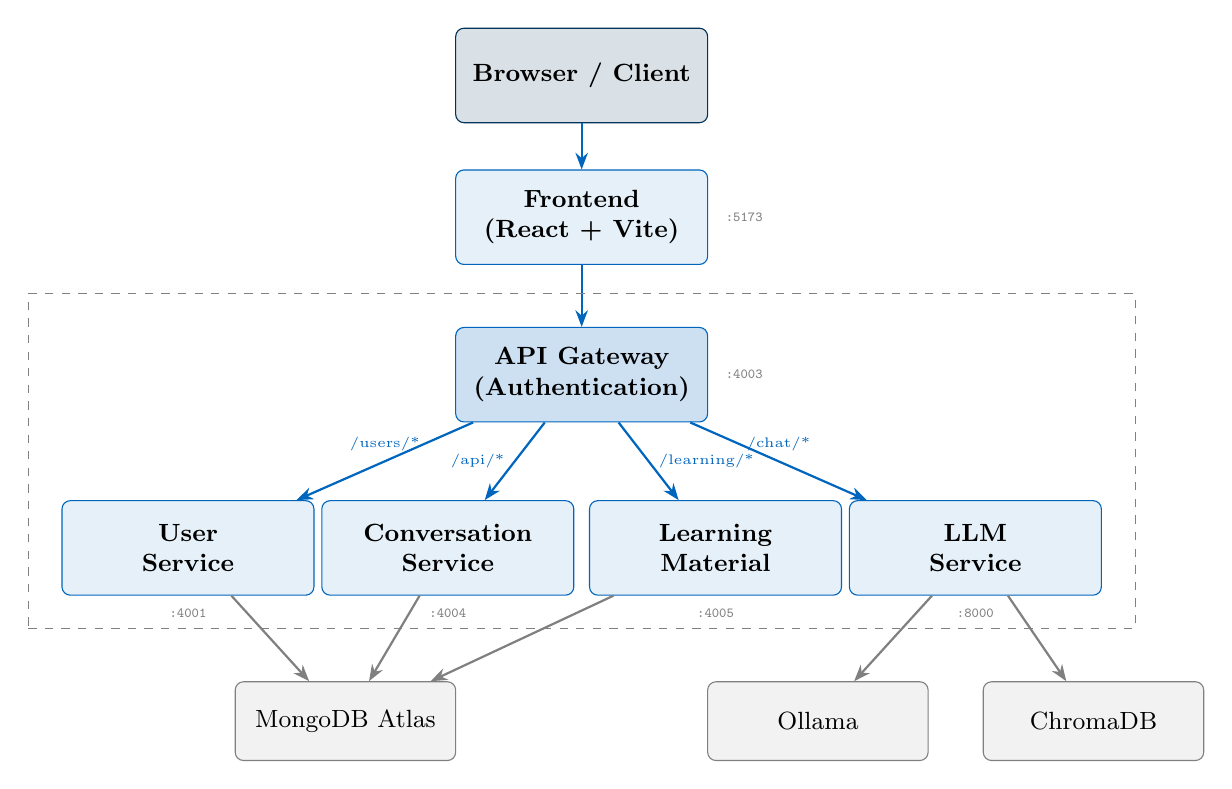
\begin{tikzpicture}[
    service/.style={rectangle, draw=TUMBlue, fill=TUMBlue!10, minimum width=3.2cm, minimum height=1.2cm, align=center, font=\small\bfseries, rounded corners=3pt},
    external/.style={rectangle, draw=gray, fill=gray!10, minimum width=2.8cm, minimum height=1cm, align=center, font=\small, rounded corners=3pt},
    arrow/.style={-{Stealth[length=6pt]}, thick, TUMBlue},
    label/.style={font=\tiny\ttfamily, color=gray}
]

% Client
\node[service, fill=TUMDarkBlue!15, draw=TUMDarkBlue] (client) at (0, 6) {Browser / Client};

% Frontend
\node[service] (frontend) at (0, 4.2) {Frontend\\(React + Vite)};
\node[label, right=0.1cm of frontend] {:5173};

% API Gateway
\node[service, fill=TUMBlue!20] (gateway) at (0, 2.2) {API Gateway\\(Authentication)};
\node[label, right=0.1cm of gateway] {:4003};

% Backend services
\node[service] (user) at (-5, 0) {User\\Service};
\node[label, below=0.05cm of user] {:4001};

\node[service] (conversation) at (-1.7, 0) {Conversation\\Service};
\node[label, below=0.05cm of conversation] {:4004};

\node[service] (learning) at (1.7, 0) {Learning\\Material};
\node[label, below=0.05cm of learning] {:4005};

\node[service] (llm) at (5, 0) {LLM\\Service};
\node[label, below=0.05cm of llm] {:8000};

% External services
\node[external] (mongodb) at (-3, -2.2) {MongoDB Atlas};
\node[external] (ollama) at (3, -2.2) {Ollama};
\node[external] (chroma) at (6.5, -2.2) {ChromaDB};

% Arrows
\draw[arrow] (client) -- (frontend);
\draw[arrow] (frontend) -- (gateway);
\draw[arrow] (gateway) -- (user) node[midway, above, font=\tiny] {/users/*};
\draw[arrow] (gateway) -- (conversation) node[midway, left, font=\tiny] {/api/*};
\draw[arrow] (gateway) -- (learning) node[midway, right, font=\tiny] {/learning/*};
\draw[arrow] (gateway) -- (llm) node[midway, above, font=\tiny] {/chat/*};
\draw[arrow, gray] (user) -- (mongodb);
\draw[arrow, gray] (conversation) -- (mongodb);
\draw[arrow, gray] (learning) -- (mongodb);
\draw[arrow, gray] (llm) -- (ollama);
\draw[arrow, gray] (llm) -- (chroma);

% Network box
\node[draw=TUMBlue, dashed, inner sep=12pt, fit=(user)(conversation)(learning)(llm)(gateway), label={[font=\small\color{TUMBlue}]below:Docker Bridge Network (atoss-network)}] {};

\end{tikzpicture}
\caption{ATOSS.GPT system architecture}
\label{fig:architecture}
\end{figure}


% ============================================================
% CHAPTER 2: INSTALLATION AND USAGE
% ============================================================
\chapter{Installation and Usage}

\section{System Requirements}

\begin{table}[H]
\centering
\begin{tabularx}{\textwidth}{lXl}
    \toprule
    \textbf{Component} & \textbf{Description} & \textbf{Minimum Version} \\
    \midrule
    Node.js & Runtime for frontend and 4 backend services & 18+ \\
    Python & Runtime for LLM service & 3.12+ \\
    MongoDB & Database (Atlas cloud or local instance) & 6.0+ \\
    Ollama & Local LLM inference server & Latest \\
    Docker \& Compose & Containerized deployment & Latest \\
    Operating System & Linux, macOS, or Windows (with WSL2) & -- \\
    RAM & For embedding model and LLM & 8 GB+ recommended \\
    Disk Space & Models, ChromaDB, and application data & 5 GB+ \\
    \bottomrule
\end{tabularx}
\caption{System requirements}
\label{tab:sysreq}
\end{table}

\section{Docker Installation (Recommended)}

\begin{enumerate}
    \item \textbf{Clone the repository:}
\begin{lstlisting}[language=bash]
git clone https://gitlab.lrz.de/seba-master-lab/atoss.gpt.git
cd atoss.gpt
\end{lstlisting}

    \item \textbf{Configure environment files:} Copy \texttt{.env.example} to \texttt{.env} in each service directory and fill in the required values:
\begin{lstlisting}[language=bash]
cp backend/authentication/.env.example backend/authentication/.env
cp backend/user/.env.example backend/user/.env
cp backend/conversation/.env.example backend/conversation/.env
cp backend/learning-material/.env.example backend/learning-material/.env
cp backend/llm/.env.example backend/llm/.env
cp frontend/.env.example frontend/.env
\end{lstlisting}

    \item \textbf{Install and start Ollama:} Download Ollama from \url{https://ollama.ai} and pull the required model:
\begin{lstlisting}[language=bash]
ollama pull qwen3:4b-instruct
\end{lstlisting}

    \item \textbf{Uncomment LLM services} (optional): In \texttt{docker-compose.yml}, uncomment the \texttt{llm} and \texttt{ollama} service blocks if you want them containerized. Otherwise, run Ollama and the LLM service locally.

    \item \textbf{Build and start all services:}
\begin{lstlisting}[language=bash]
docker-compose up --build
\end{lstlisting}

    \item \textbf{Access the application:} Open \url{http://localhost:5173} in your browser.
\end{enumerate}

\section{Manual Installation}

If you prefer to run services individually without Docker:

\subsection{Frontend (Port 5173)}
\begin{lstlisting}[language=bash]
cd frontend
npm install
npm run dev
\end{lstlisting}

\subsection{Authentication Service / API Gateway (Port 4003)}
\begin{lstlisting}[language=bash]
cd backend/authentication
npm install
node index.js
\end{lstlisting}

\subsection{User Service (Port 4001)}
\begin{lstlisting}[language=bash]
cd backend/user
npm install
node index.js
\end{lstlisting}

\subsection{Conversation Service (Port 4004)}
\begin{lstlisting}[language=bash]
cd backend/conversation
npm install
node index.js
\end{lstlisting}

\subsection{Learning Material Service (Port 4005)}
\begin{lstlisting}[language=bash]
cd backend/learning-material
npm install
node index.js
\end{lstlisting}

\subsection{LLM Service (Port 8000)}
\begin{lstlisting}[language=bash]
cd backend/llm
pip install -r requirements.txt
python main.py
\end{lstlisting}

\textbf{Note:} Ollama must be running locally before starting the LLM service. Ensure the \texttt{OLLAMA\_BASE\_URL} in \texttt{backend/llm/.env} points to \texttt{http://localhost:11434} for local development.

\section{Configuration Reference}

Each microservice is configured via environment variables in its respective \texttt{.env} file.

\subsection{Authentication Service}
\begin{table}[H]
\centering
\begin{tabularx}{\textwidth}{lX}
    \toprule
    \textbf{Variable} & \textbf{Description} \\
    \midrule
    \texttt{PORT} & Server port (default: 4003) \\
    \texttt{MONGODB\_URI} & MongoDB connection string \\
    \texttt{JWT\_SECRET} & Secret key for JWT token signing \\
    \texttt{JWT\_EXPIRATION} & Token expiration time (default: 24h) \\
    \texttt{REFRESH\_TOKEN\_SECRET} & Secret key for refresh tokens \\
    \texttt{USER\_SERVICE\_URL} & URL of the User Service \\
    \texttt{CHATBOT\_SERVICE\_URL} & URL of the LLM Service \\
    \texttt{LEARNING\_SERVICE\_URL} & URL of the Learning Material Service \\
    \texttt{FRONTEND\_URL} & Frontend URL for CORS \\
    \texttt{APP\_URL} & Application URL for email links \\
    \texttt{SMTP\_HOST} & SMTP server host (default: smtp.gmail.com) \\
    \texttt{SMTP\_PORT} & SMTP server port (default: 587) \\
    \texttt{SMTP\_USER} & SMTP username \\
    \texttt{SMTP\_PASS} & SMTP password (app-specific password) \\
    \texttt{EMAIL\_FROM} & Sender email address \\
    \bottomrule
\end{tabularx}
\caption{Authentication service environment variables}
\end{table}

\subsection{LLM Service}
\begin{table}[H]
\centering
\begin{tabularx}{\textwidth}{lX}
    \toprule
    \textbf{Variable} & \textbf{Description} \\
    \midrule
    \texttt{HOST} & Server host (default: 0.0.0.0) \\
    \texttt{PORT} & Server port (default: 8000) \\
    \texttt{OLLAMA\_BASE\_URL} & Ollama server URL \\
    \texttt{OLLAMA\_MODEL} & LLM model name (default: qwen3:4b-instruct) \\
    \texttt{OLLAMA\_TEMPERATURE} & Generation temperature (default: 0.3) \\
    \texttt{OLLAMA\_NUM\_CTX} & Context window size (default: 20000) \\
    \texttt{OLLAMA\_REPEAT\_PENALTY} & Repetition penalty (default: 1.15) \\
    \texttt{OLLAMA\_NUM\_PREDICT} & Max tokens to generate (default: 1000) \\
    \texttt{OLLAMA\_KEEP\_ALIVE} & Keep model loaded (default: -1, forever) \\
    \texttt{EMBEDDING\_MODEL} & Embedding model (Snowflake/snowflake-arctic-embed-l-v2.0) \\
    \texttt{EMBEDDING\_DEVICE} & Compute device (auto/cuda/mps/cpu) \\
    \texttt{CHROMA\_PERSIST\_DIRECTORY} & ChromaDB storage path \\
    \texttt{CHROMA\_COLLECTION\_NAME} & ChromaDB collection (default: tum\_docs) \\
    \texttt{ENABLE\_RERANKING} & Enable document reranking (default: false) \\
    \texttt{RERANKING\_MODEL} & Reranker model name \\
    \texttt{RERANKING\_TOP\_K} & Number of documents after reranking (default: 5) \\
    \bottomrule
\end{tabularx}
\caption{LLM service environment variables}
\end{table}

\subsection{Other Services}
The User Service (\texttt{PORT}, \texttt{MONGODB\_URI}), Conversation Service (\texttt{PORT}, \texttt{MONGODB\_URI}, \texttt{CHATBOT\_SERVICE\_URL}), and Learning Material Service (\texttt{PORT}, \texttt{MONGODB\_URI}) each require their port and MongoDB connection string.

The Frontend uses \texttt{VITE\_}-prefixed variables: \texttt{VITE\_AUTH\_LOGIN\_URL}, \texttt{VITE\_USER\_SERVICE\_URL}, \texttt{VITE\_CONVERSATION\_URL}, \texttt{VITE\_LEARNING\_API\_URL}, and \texttt{VITE\_IMAGE\_BASE\_URL}.

\section{Starting and Stopping}

\subsection{With Docker Compose}
\begin{lstlisting}[language=bash]
# Start all services (detached)
docker-compose up -d

# View logs
docker-compose logs -f

# Stop all services
docker-compose down

# Rebuild after code changes
docker-compose up --build -d
\end{lstlisting}

\subsection{Health Checks}
\begin{itemize}
    \item API Gateway: \texttt{GET http://localhost:4003/api/health}
    \item LLM Service: \texttt{GET http://localhost:8000/api/chat/health}
    \item LLM Status: \texttt{GET http://localhost:8000/api/chat/status} -- returns component loading status
\end{itemize}

\section{User Guide}

\subsection{Registration and Login}
\begin{enumerate}
    \item Navigate to the application at \texttt{http://localhost:5173}.
    \item Click \textbf{Register} to create a new account. A valid TUM email address is required (\texttt{@tum.de}, \texttt{@mytum.de}, or \texttt{@mri.tum.de}).
    \item Select your department and choose a strong password (minimum 8 characters with letters and numbers).
    \item After registration, check your email for a verification link and click it.
    \item Return to the login page and sign in with your credentials.
\end{enumerate}

% Screenshot placeholder
\begin{figure}[H]
\centering
\fbox{\parbox{0.7\textwidth}{\centering\vspace{3cm}\textit{Screenshot: Login Page}\vspace{3cm}}}
\caption{Login page}
\label{fig:login}
\end{figure}

\subsection{Using the Chatbot}
\begin{enumerate}
    \item After login, you are directed to the \textbf{Chatbot} page (\texttt{/chatbot}).
    \item Type your question about ATOSS Staff Center in the message input field (German language).
    \item Press Enter or click Send. The AI response streams in real-time.
    \item Responses include source references and may contain embedded screenshots from the documentation.
    \item Use the \textbf{sidebar} to manage conversations: create new chats, search history, rename, or delete conversations.
\end{enumerate}

\begin{figure}[H]
\centering
\fbox{\parbox{0.7\textwidth}{\centering\vspace{3cm}\textit{Screenshot: Chat Interface}\vspace{3cm}}}
\caption{Chatbot interface with streaming response}
\label{fig:chatbot}
\end{figure}

\subsection{Analytics Dashboard}
Navigate to \texttt{/analytics} to view:
\begin{itemize}
    \item \textbf{Keyword frequency} charts showing the most common query terms
    \item \textbf{Category breakdown} pie charts (e.g., Zeitwirtschaft, Dienstplanung)
    \item \textbf{Timeline analysis} of query volume over time
    \item Use \textbf{date range filters} to narrow the analysis period
    \item Click \textbf{Export CSV} to download raw analytics data
    \item Click \textbf{Process Queries} to analyze new unprocessed queries
\end{itemize}

\subsection{Learning Materials}
Navigate to \texttt{/learning} to browse video tutorials:
\begin{itemize}
    \item Browse videos by category or search by title
    \item Click a video card to open the player modal
    \item Admin users can upload, edit, and delete videos via the management interface
\end{itemize}

\subsection{User Profile}
Navigate to \texttt{/profile} to manage:
\begin{itemize}
    \item Profile picture (upload or remove)
    \item Username and department
    \item Theme preference (light, dark, or auto)
    \item Language and notification settings
    \item Password change
    \item Account deletion
\end{itemize}

\section{Troubleshooting}

\errorbox{%
\textbf{Ollama Connection Refused}\\[4pt]
\textbf{Error:} \texttt{Connection refused} when starting the LLM service.\\
\textbf{Solution:} Ensure Ollama is running (\texttt{ollama serve}) and the \texttt{OLLAMA\_BASE\_URL} in \texttt{backend/llm/.env} matches the Ollama address. For Docker, use \texttt{http://ollama:11434}; for local development, use \texttt{http://localhost:11434}.%
}

\errorbox{%
\textbf{Vector Store Not Found}\\[4pt]
\textbf{Error:} LLM service reports vector store not loaded.\\
\textbf{Solution:} Ensure the ChromaDB directory (\texttt{chroma\_db\_merged/}) exists in \texttt{backend/llm/} and contains ingested documents. Run the ingestion pipeline first if the directory is empty.%
}

\errorbox{%
\textbf{Email Verification Not Received}\\[4pt]
\textbf{Error:} No verification email after registration.\\
\textbf{Solution:} Check the SMTP configuration in \texttt{backend/authentication/.env}. Ensure the Gmail account has an app-specific password configured and ``Less secure app access'' is enabled if needed.%
}

\warnbox{%
\textbf{MongoDB Connection Issues}\\[4pt]
\textbf{Error:} Services fail to connect to MongoDB.\\
\textbf{Solution:} Verify the \texttt{MONGODB\_URI} in each service's \texttt{.env} file. For MongoDB Atlas, ensure your IP address is whitelisted in the Atlas Network Access settings.%
}

\warnbox{%
\textbf{CORS Errors in Browser}\\[4pt]
\textbf{Error:} Cross-origin requests blocked in the browser console.\\
\textbf{Solution:} Ensure the \texttt{FRONTEND\_URL} in the authentication service matches the actual frontend URL (e.g., \texttt{http://localhost:5173}).%
}


% ============================================================
% CHAPTER 3: DEVELOPER DOCUMENTATION
% ============================================================
\chapter{Developer Documentation}

\section{Project Structure}

\begin{lstlisting}[basicstyle=\ttfamily\footnotesize, frame=none, numbers=none, backgroundcolor=\color{white}]
atoss.gpt/
|-- frontend/                     # React + Vite frontend
|   |-- src/
|   |   |-- components/           # 11 reusable UI components
|   |   |-- pages/                # 8 page components
|   |   |-- services/             # API integration (axios)
|   |   |-- utils/                # Validation helpers
|   |   |-- assets/               # Images and static assets
|   |   |-- App.jsx               # Router configuration
|   |   +-- main.jsx              # Entry point
|   |-- public/                   # Static assets
|   |-- Dockerfile                # Multi-stage build (Node -> Nginx)
|   +-- nginx.conf                # SPA routing config
|
|-- backend/
|   |-- authentication/           # API Gateway + Auth (Port 4003)
|   |   |-- controllers/          # AuthController
|   |   |-- services/             # AuthService, EmailService
|   |   |-- models/               # UserCredentials, Role, Department
|   |   |-- middleware/            # authMiddleware, gatewayMiddleware
|   |   |-- gateway/              # apiGateway (proxy routing)
|   |   +-- routes/               # authRoutes
|   |
|   |-- user/                     # User Profile Service (Port 4001)
|   |   |-- controllers/          # UserController
|   |   |-- services/             # UserService
|   |   |-- models/               # UserProfile, Role
|   |   +-- routes/               # userRoutes
|   |
|   |-- conversation/             # Conversation & Analytics (Port 4004)
|   |   |-- controllers/          # conversation, message, analytics
|   |   |-- services/             # conversation, message, analytics, llmClassification
|   |   |-- models/               # Conversation, Message, QueryAnalytics
|   |   +-- routes/               # conversation, message, analytics
|   |
|   |-- learning-material/        # Video Management (Port 4005)
|   |   |-- controllers/          # videoController
|   |   |-- services/             # videoService
|   |   |-- models/               # Video
|   |   |-- routes/               # videoRoutes
|   |   +-- uploads/              # Video and thumbnail storage
|   |
|   |-- llm/                      # RAG Pipeline (Port 8000)
|   |   |-- controllers/          # chat_controller
|   |   |-- services/             # rag_chain, startup, docling, image_storage
|   |   |-- models/               # embedding, llm, vectorstore, reranker
|   |   |-- routes/               # chat_routes
|   |   |-- config/               # settings (pydantic)
|   |   |-- docling/              # PDF/PPTX document processing
|   |   +-- chroma_db_merged/     # ChromaDB vector store data
|   |
|   +-- ingestion/                # Data ingestion utilities
|
|-- docker-compose.yml            # Service orchestration
|-- README.md                     # Quick start guide
+-- doc/                          # Internal technical documentation
\end{lstlisting}

\section{Technologies and Versions}

\begin{table}[H]
\centering
\caption{Frontend technologies}
\begin{tabularx}{\textwidth}{llX}
    \toprule
    \textbf{Technology} & \textbf{Version} & \textbf{Purpose} \\
    \midrule
    React & 19.1.1 & UI component framework \\
    Vite & 7.1.7 & Build tool and dev server \\
    Tailwind CSS & 3.4.18 & Utility-first CSS framework \\
    React Router & 6.30.2 & Client-side routing \\
    Axios & 1.13.1 & HTTP client \\
    Plotly.js & 2.30.0 & Data visualization (analytics) \\
    react-markdown & 10.1.0 & Markdown rendering in chat \\
    react-toastify & 11.0.5 & Toast notifications \\
    \bottomrule
\end{tabularx}
\end{table}

\begin{table}[H]
\centering
\caption{Backend technologies (Node.js services)}
\begin{tabularx}{\textwidth}{llX}
    \toprule
    \textbf{Technology} & \textbf{Version} & \textbf{Purpose} \\
    \midrule
    Express.js & 5.1.0 & HTTP server framework \\
    Mongoose & 8.19.2+ & MongoDB ODM \\
    jsonwebtoken & 9.0.2 & JWT authentication \\
    bcryptjs & 2.4.3 & Password hashing \\
    express-http-proxy & 2.0.0 & API Gateway proxying \\
    nodemailer & 6.9.16 & Email sending (verification) \\
    multer & 1.4.5 & File upload handling \\
    morgan & 1.10.1 & HTTP request logging \\
    \bottomrule
\end{tabularx}
\end{table}

\begin{table}[H]
\centering
\caption{Backend technologies (Python LLM service)}
\begin{tabularx}{\textwidth}{llX}
    \toprule
    \textbf{Technology} & \textbf{Version} & \textbf{Purpose} \\
    \midrule
    FastAPI & $\geq$0.115.0 & Async API framework \\
    Uvicorn & $\geq$0.32.0 & ASGI server \\
    ChromaDB & 1.3.5 & Vector store for document embeddings \\
    sentence-transformers & 5.1.2 & Embedding model loading \\
    ollama (Python) & 0.6.1 & LLM client library \\
    pydantic-settings & $\geq$2.6.0 & Configuration management \\
    aiohttp / httpx & $\geq$3.10.0 / $\geq$0.27.0 & Async HTTP clients \\
    \bottomrule
\end{tabularx}
\end{table}

\section{Build and Deployment}

The project uses \textbf{Docker Compose} for orchestration. All services are connected via a custom bridge network (\texttt{atoss-network}).

\begin{table}[H]
\centering
\caption{Docker Compose services}
\begin{tabularx}{\textwidth}{llllX}
    \toprule
    \textbf{Service} & \textbf{Port} & \textbf{Image Base} & \textbf{Status} & \textbf{Dependencies} \\
    \midrule
    frontend & 5173 & Node 18 $\rightarrow$ Nginx & Active & authentication, conversation \\
    authentication & 4003 & Node 18 Alpine & Active & -- \\
    user & 4001 & Node 18 Alpine & Active & authentication \\
    conversation & 4004 & Node 18 Alpine & Active & authentication \\
    learning-material & 4005 & Node 18 Alpine & Active & authentication \\
    llm & 8000 & Python & Disabled & ollama \\
    ollama & 11434 & ollama/ollama & Disabled & -- \\
    \bottomrule
\end{tabularx}
\end{table}

\textbf{Volumes:}
\begin{itemize}
    \item \texttt{ollama\_data} -- Persists downloaded Ollama models
    \item \texttt{hf\_cache} -- Caches Hugging Face embedding models
    \item \texttt{./backend/learning-material/uploads/} -- Persists uploaded videos and thumbnails
\end{itemize}

All services use \texttt{restart: unless-stopped} policy. The LLM service has a health check with a 180-second start period to allow model loading.

\section{Architecture}

\subsection{API Gateway Pattern}

The Authentication Service (port 4003) acts as both the authentication provider and the API Gateway. It handles \texttt{/auth/*} routes locally and proxies all other requests to the appropriate microservice:

\begin{table}[H]
\centering
\begin{tabularx}{\textwidth}{lllX}
    \toprule
    \textbf{Route Pattern} & \textbf{Target Service} & \textbf{Target Port} & \textbf{Description} \\
    \midrule
    \texttt{/auth/*} & Local & 4003 & Authentication endpoints \\
    \texttt{/users/*} & User Service & 4001 & User profile management \\
    \texttt{/chat/*} & LLM Service & 8000 & Chat and RAG endpoints \\
    \texttt{/learning/*} & Conversation Service & 4004 & Learning material (Note: proxied to conversation) \\
    \texttt{/api/health} & Local & 4003 & Health check \\
    \bottomrule
\end{tabularx}
\caption{API Gateway routing}
\end{table}

\subsection{Authentication Flow}

\begin{enumerate}
    \item User submits credentials to \texttt{POST /auth/login}.
    \item \texttt{AuthService} verifies email/password and checks email verification status.
    \item On success, a JWT access token (24h expiry) and refresh token are generated and returned.
    \item The frontend stores tokens in \texttt{localStorage}.
    \item All subsequent requests include the \texttt{Authorization: Bearer <token>} header.
    \item The \texttt{gatewayMiddleware} validates tokens on protected routes before proxying.
    \item When the access token expires, the frontend calls \texttt{POST /auth/refresh} with the refresh token.
\end{enumerate}

\subsection{Chat Message Flow}

\begin{figure}[H]
\centering
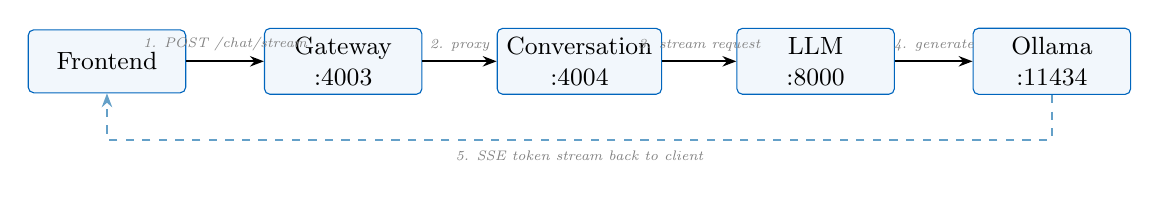
\begin{tikzpicture}[
    box/.style={rectangle, draw=TUMBlue, fill=TUMBlue!5, minimum width=2cm, minimum height=0.8cm, align=center, font=\small, rounded corners=2pt},
    arrow/.style={-{Stealth[length=5pt]}, thick},
    note/.style={font=\tiny\itshape, text=gray}
]

\node[box] (fe) at (0,0) {Frontend};
\node[box] (gw) at (3,0) {Gateway\\:4003};
\node[box] (conv) at (6,0) {Conversation\\:4004};
\node[box] (llm) at (9,0) {LLM\\:8000};
\node[box] (oll) at (12,0) {Ollama\\:11434};

% Forward flow
\draw[arrow] (fe) -- (gw) node[midway, above, note] {1. POST /chat/stream};
\draw[arrow] (gw) -- (conv) node[midway, above, note] {2. proxy};
\draw[arrow] (conv) -- (llm) node[midway, above, note] {3. stream request};
\draw[arrow] (llm) -- (oll) node[midway, above, note] {4. generate};

% Return flow (SSE)
\draw[arrow, dashed, TUMLightBlue] (oll) -- ++(0,-1) -| (fe) node[pos=0.25, below, note] {5. SSE token stream back to client};

\end{tikzpicture}
\caption{Chat message flow (simplified)}
\label{fig:chatflow}
\end{figure}

\section{Database Structure}

The application uses \textbf{MongoDB} with six collections across the microservices. All services connect to the same MongoDB Atlas cluster.

\begin{figure}[H]
\centering
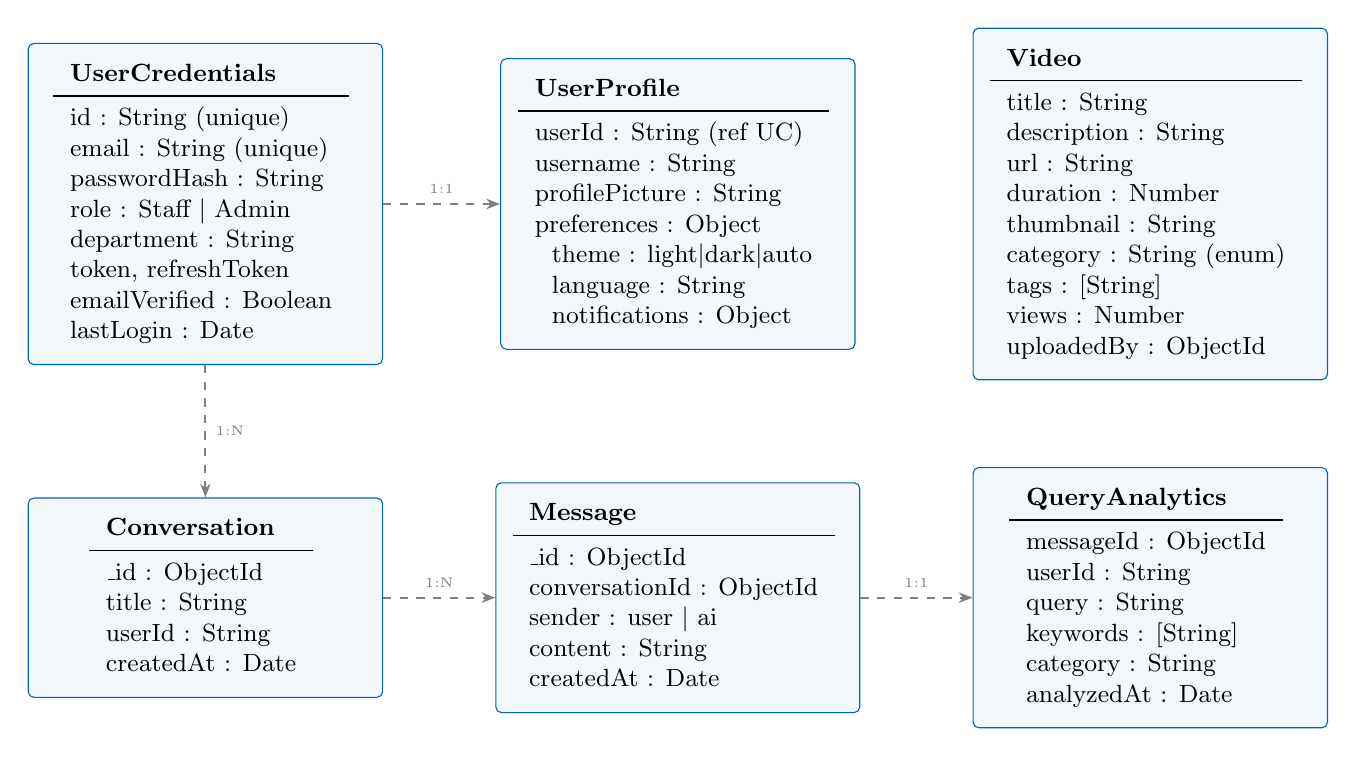
\begin{tikzpicture}[
    entity/.style={rectangle, draw=TUMBlue, fill=TUMBlue!5, minimum width=4.5cm, align=left, font=\small, inner sep=6pt, rounded corners=2pt},
    title/.style={font=\small\bfseries\color{TUMDarkBlue}},
    rel/.style={-{Stealth[length=5pt]}, thick, gray, dashed}
]

% UserCredentials
\node[entity] (uc) at (0, 0) {
    \begin{tabular}{l}
    \textbf{UserCredentials} \\
    \midrule
    id : String (unique) \\
    email : String (unique) \\
    passwordHash : String \\
    role : Staff $|$ Admin \\
    department : String \\
    token, refreshToken \\
    emailVerified : Boolean \\
    lastLogin : Date \\
    \end{tabular}
};

% UserProfile
\node[entity] (up) at (6, 0) {
    \begin{tabular}{l}
    \textbf{UserProfile} \\
    \midrule
    userId : String (ref UC) \\
    username : String \\
    profilePicture : String \\
    preferences : Object \\
    ~~theme : light$|$dark$|$auto \\
    ~~language : String \\
    ~~notifications : Object \\
    \end{tabular}
};

% Conversation
\node[entity] (conv) at (0, -5) {
    \begin{tabular}{l}
    \textbf{Conversation} \\
    \midrule
    \_id : ObjectId \\
    title : String \\
    userId : String \\
    createdAt : Date \\
    \end{tabular}
};

% Message
\node[entity] (msg) at (6, -5) {
    \begin{tabular}{l}
    \textbf{Message} \\
    \midrule
    \_id : ObjectId \\
    conversationId : ObjectId \\
    sender : user $|$ ai \\
    content : String \\
    createdAt : Date \\
    \end{tabular}
};

% QueryAnalytics
\node[entity] (qa) at (12, -5) {
    \begin{tabular}{l}
    \textbf{QueryAnalytics} \\
    \midrule
    messageId : ObjectId \\
    userId : String \\
    query : String \\
    keywords : [String] \\
    category : String \\
    analyzedAt : Date \\
    \end{tabular}
};

% Video
\node[entity] (vid) at (12, 0) {
    \begin{tabular}{l}
    \textbf{Video} \\
    \midrule
    title : String \\
    description : String \\
    url : String \\
    duration : Number \\
    thumbnail : String \\
    category : String (enum) \\
    tags : [String] \\
    views : Number \\
    uploadedBy : ObjectId \\
    \end{tabular}
};

% Relationships
\draw[rel] (uc.east) -- (up.west) node[midway, above, font=\tiny] {1:1};
\draw[rel] (conv.east) -- (msg.west) node[midway, above, font=\tiny] {1:N};
\draw[rel] (msg.east) -- (qa.west) node[midway, above, font=\tiny] {1:1};
\draw[rel] (uc.south) -- (conv.north) node[midway, right, font=\tiny] {1:N};

\end{tikzpicture}
\caption{MongoDB collections and relationships (ER diagram)}
\label{fig:er-diagram}
\end{figure}

\section{API Reference}

\subsection{Authentication Service (\texttt{/auth}, Port 4003)}

\begin{longtable}{llcp{5.5cm}}
    \toprule
    \textbf{Method} & \textbf{Endpoint} & \textbf{Auth} & \textbf{Description} \\
    \midrule
    \endhead
    POST & /auth/login & No & Login with email and password \\
    POST & /auth/register & No & Register new user \\
    POST & /auth/refresh & No & Refresh JWT access token \\
    GET & /auth/verify & No & Verify token validity \\
    POST & /auth/verify-email & No & Verify email with token \\
    POST & /auth/resend-verification & No & Resend verification email \\
    POST & /auth/logout & Yes & Logout and invalidate tokens \\
    GET & /auth/user/:userId & Yes & Get user by ID \\
    GET & /auth/user/email/:email & Yes & Get user by email \\
    PATCH & /auth/user/:userId/role & Yes & Update user role \\
    PATCH & /auth/user/:userId/department & Yes & Update department \\
    PATCH & /auth/user/:userId/password & Yes & Change password \\
    DELETE & /auth/user/:userId & Yes & Delete user account \\
    \bottomrule
\caption{Authentication Service API endpoints}
\end{longtable}

\subsection{User Service (\texttt{/users}, Port 4001)}

\begin{longtable}{llcp{5.5cm}}
    \toprule
    \textbf{Method} & \textbf{Endpoint} & \textbf{Auth} & \textbf{Description} \\
    \midrule
    \endhead
    GET & /users/:userId/verify & No & Verify user existence \\
    GET & /users/me & Yes & Get current user profile \\
    PATCH & /users/me/username & Yes & Update username \\
    PATCH & /users/me/role & Yes & Update role \\
    PATCH & /users/me/department & Yes & Update department \\
    PATCH & /users/me/password & Yes & Change password \\
    PATCH & /users/me/preferences & Yes & Update preferences \\
    PATCH & /users/me/profile-picture & Yes & Upload profile picture \\
    DELETE & /users/me/profile-picture & Yes & Remove profile picture \\
    DELETE & /users/me & Yes & Delete account \\
    POST & /users/add-admin & Yes & Promote user to admin \\
    \bottomrule
\caption{User Service API endpoints}
\end{longtable}

\subsection{Conversation Service (\texttt{/api/conversations}, Port 4004)}

\begin{longtable}{lp{5cm}p{5.5cm}}
    \toprule
    \textbf{Method} & \textbf{Endpoint} & \textbf{Description} \\
    \midrule
    \endhead
    POST & /api/conversations & Create new conversation \\
    GET & /api/conversations/user/:userId & Get all user conversations \\
    GET & /api/conversations/:id & Get conversation by ID \\
    PUT & /api/conversations/:id & Update conversation title \\
    DELETE & /api/conversations/:id & Delete conversation \\
    GET & /api/conversations/:id/stream & Stream AI response (SSE) \\
    POST & /api/conversations/:id/messages/batch & Batch save messages \\
    POST & /api/conversations/:id/messages & Create single message \\
    GET & /api/conversations/:id/messages & Get conversation messages \\
    DELETE & /api/conversations/messages/:msgId & Delete a message \\
    \bottomrule
\caption{Conversation Service API endpoints}
\end{longtable}

\subsection{Analytics Service (\texttt{/api/analytics}, Port 4004)}

\begin{longtable}{llp{6cm}}
    \toprule
    \textbf{Method} & \textbf{Endpoint} & \textbf{Description} \\
    \midrule
    \endhead
    POST & /api/analytics/process & Process unanalyzed queries \\
    GET & /api/analytics/keywords & Keyword frequency statistics \\
    GET & /api/analytics/categories & Category distribution \\
    GET & /api/analytics/timeline & Query volume over time \\
    GET & /api/analytics/overall & Overall statistics summary \\
    GET & /api/analytics/dashboard & Complete dashboard data \\
    GET & /api/analytics/export & Export queries as CSV \\
    \bottomrule
\caption{Analytics API endpoints}
\end{longtable}

\subsection{Learning Material Service (\texttt{/api/videos}, Port 4005)}

\begin{longtable}{llp{6cm}}
    \toprule
    \textbf{Method} & \textbf{Endpoint} & \textbf{Description} \\
    \midrule
    \endhead
    GET & /api/videos & Get all videos \\
    POST & /api/videos & Upload video (multipart/form-data) \\
    GET & /api/videos/:id & Get video by ID \\
    PUT & /api/videos/:id & Update video metadata \\
    DELETE & /api/videos/:id & Delete video \\
    POST & /api/videos/:id/view & Increment view count \\
    \bottomrule
\caption{Learning Material Service API endpoints}
\end{longtable}

\subsection{LLM Service (\texttt{/api/chat}, Port 8000)}

\begin{longtable}{llp{6cm}}
    \toprule
    \textbf{Method} & \textbf{Endpoint} & \textbf{Description} \\
    \midrule
    \endhead
    GET & /api/chat/status & Service and component status \\
    POST & /api/chat/generate & Generate complete response \\
    POST & /api/chat/stream & Stream response via SSE \\
    GET & /api/chat/health & Health check \\
    GET & / & Root endpoint with service info \\
    \bottomrule
\caption{LLM Service API endpoints}
\end{longtable}

\textbf{Chat Request Schema:}
\begin{lstlisting}[language=Python]
{
    "message": "Wie erstelle ich einen Dienstplan?",
    "conversation_id": "optional-id",
    "conversation_history": [
        {"role": "user", "content": "..."},
        {"role": "assistant", "content": "..."}
    ]
}
\end{lstlisting}

\section{Key Classes and Logic}

\subsection{Authentication Service}

\begin{itemize}
    \item \textbf{AuthController} -- Handles HTTP requests for login, registration, token management, and user CRUD operations.
    \item \textbf{AuthService} -- Business logic for credential verification, JWT generation (access + refresh tokens), email verification token management, and password hashing with bcryptjs.
    \item \textbf{EmailService} -- Sends verification emails via Nodemailer using Gmail SMTP.
    \item \textbf{gatewayMiddleware} -- Validates JWT tokens on protected routes; skips validation for public routes (login, register, verify).
    \item \textbf{apiGateway} -- Configures \texttt{express-http-proxy} to route requests to downstream services, forwarding the Authorization header.
\end{itemize}

\subsection{Conversation Service}

\begin{itemize}
    \item \textbf{ConversationService} -- CRUD operations for conversations. Creates conversations with auto-generated titles.
    \item \textbf{MessageService} -- Manages individual messages within conversations.
    \item \textbf{AnalyticsService} -- Processes user queries by extracting keywords and assigning categories using the LLM classification service. Aggregates data for dashboard visualization.
    \item \textbf{LLMClassificationService} -- Uses the LLM to classify queries into predefined categories (Zeitwirtschaft, Dienstplanung, Prozessfragen, etc.) and extract meaningful keywords.
\end{itemize}

\subsection{LLM Service (Python)}

\begin{itemize}
    \item \textbf{StartupService} -- Initializes all components on server start: embedding model, vector store, LLM connection, and optional reranker. Reports loading progress.
    \item \textbf{EmbeddingManager} (Singleton) -- Loads and manages the Snowflake Arctic Embed L v2.0 model for query and document embedding.
    \item \textbf{VectorStoreManager} (Singleton) -- Manages ChromaDB connection, collection switching, and similarity search (k=8 documents).
    \item \textbf{LLMManager} (Singleton) -- Interfaces with Ollama for text generation and streaming. Configures the German-language system prompt for TUM hospital context.
    \item \textbf{RAGChainService} (Singleton) -- Orchestrates the full RAG pipeline: retrieves documents, optionally reranks them, formats context, and generates responses with source citations.
    \item \textbf{RerankerManager} (Singleton) -- Optional Jina Reranker v3 for improving retrieval quality (disabled by default).
\end{itemize}

\section{RAG Pipeline}

The Retrieval-Augmented Generation pipeline is the core of the chatbot's intelligence. It operates in two phases:

\begin{figure}[H]
\centering
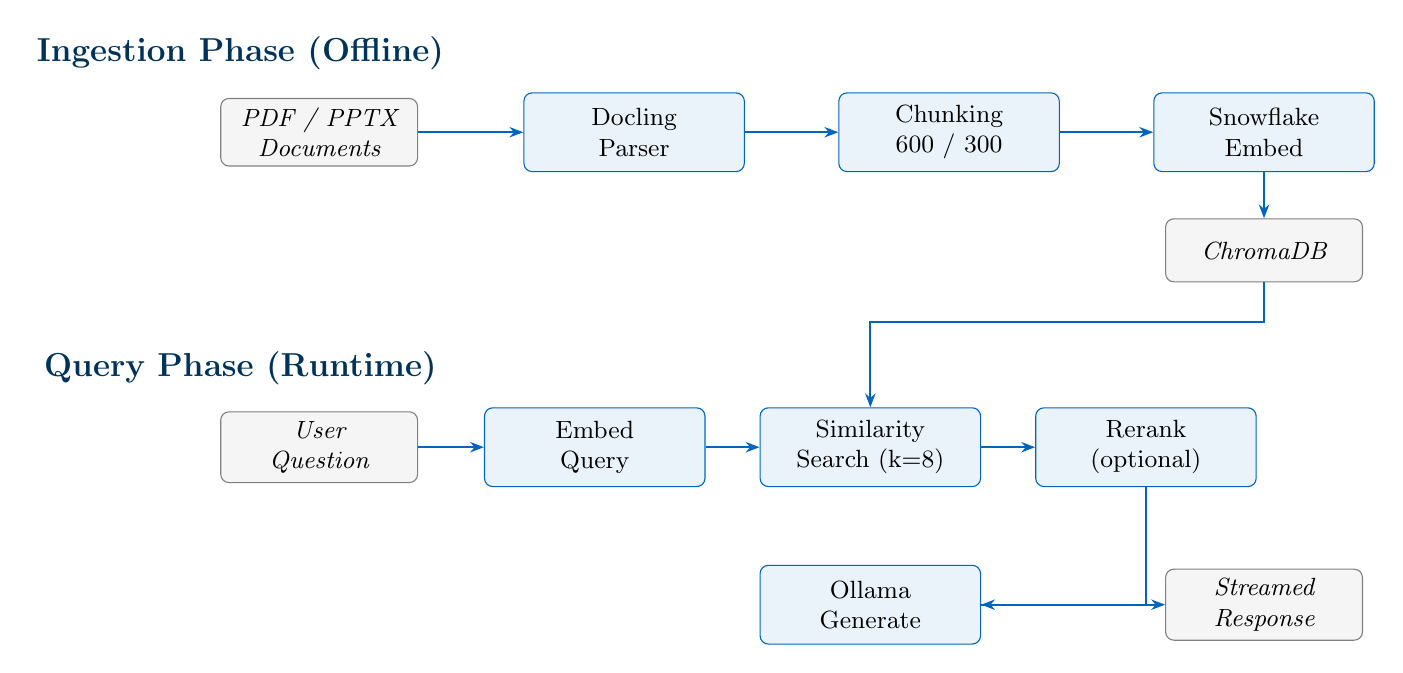
\begin{tikzpicture}[
    proc/.style={rectangle, draw=TUMBlue, fill=TUMBlue!8, minimum width=2.8cm, minimum height=1cm, align=center, font=\small, rounded corners=3pt},
    data/.style={rectangle, draw=gray, fill=gray!8, minimum width=2.5cm, minimum height=0.8cm, align=center, font=\small\itshape, rounded corners=3pt},
    arrow/.style={-{Stealth[length=5pt]}, thick, TUMBlue},
    phase/.style={font=\large\bfseries\color{TUMDarkBlue}}
]

% Ingestion Phase
\node[phase] at (-1, 5.5) {Ingestion Phase (Offline)};
\node[data] (docs) at (0, 4.5) {PDF / PPTX\\Documents};
\node[proc] (parse) at (4, 4.5) {Docling\\Parser};
\node[proc] (chunk) at (8, 4.5) {Chunking\\600 / 300};
\node[proc] (embed1) at (12, 4.5) {Snowflake\\Embed};
\node[data] (chroma) at (12, 3) {ChromaDB};

\draw[arrow] (docs) -- (parse);
\draw[arrow] (parse) -- (chunk);
\draw[arrow] (chunk) -- (embed1);
\draw[arrow] (embed1) -- (chroma);

% Query Phase
\node[phase] at (-1, 1.5) {Query Phase (Runtime)};
\node[data] (query) at (0, 0.5) {User\\Question};
\node[proc] (embed2) at (3.5, 0.5) {Embed\\Query};
\node[proc] (search) at (7, 0.5) {Similarity\\Search (k=8)};
\node[proc] (rerank) at (10.5, 0.5) {Rerank\\(optional)};
\node[proc] (gen) at (7, -1.5) {Ollama\\Generate};
\node[data] (resp) at (12, -1.5) {Streamed\\Response};

\draw[arrow] (query) -- (embed2);
\draw[arrow] (embed2) -- (search);
\draw[arrow] (search) -- (rerank);
\draw[arrow] (chroma.south) -- ++(0,-0.5) -| (search.north);
\draw[arrow] (rerank) |- (gen);
\draw[arrow] (gen) -- (resp);

\end{tikzpicture}
\caption{RAG pipeline architecture}
\label{fig:rag-pipeline}
\end{figure}

\textbf{Key Configuration:}
\begin{itemize}
    \item \textbf{Embedding Model:} Snowflake/snowflake-arctic-embed-l-v2.0
    \item \textbf{Chunk Size:} 600 characters with 300 character overlap
    \item \textbf{Retrieval:} Top 8 most similar documents from ChromaDB
    \item \textbf{Reranking:} Jina Reranker v3 (optional, reduces to top 5)
    \item \textbf{LLM:} Ollama with qwen3:4b-instruct (temperature 0.3, context window 20,000 tokens)
    \item \textbf{Fallback:} If no relevant documents found, returns: ``Auf diese Frage habe ich leider keine Antwort. Bitte wenden Sie sich an ATOSS.pa@mri.tum.de''
\end{itemize}

\section{Testing}

There is currently \textbf{no automated test framework} in the project. Testing has been performed via:

\begin{itemize}
    \item \textbf{Manual API Testing:} A Postman collection is available at \texttt{backend/authentication/ATOSS\_GPT\_Auth.postman\_collection.json} for testing authentication endpoints.
    \item \textbf{LLM Benchmarking:} Benchmark scripts exist at \texttt{backend/llm/benchmark/} for evaluating RAG pipeline accuracy and latency.
    \item \textbf{Manual UI Testing:} Frontend features tested manually via the browser.
\end{itemize}

\textbf{Recommendation for future development:} Implement Jest for Node.js services and pytest for the Python LLM service.

\section{Known Bugs and Open TODOs}

\begin{table}[H]
\centering
\begin{tabularx}{\textwidth}{lX}
    \toprule
    \textbf{Type} & \textbf{Description} \\
    \midrule
    Bug & Debug middleware logging all requests remains in conversation service \texttt{index.js} \\
    Bug & Exception handling order in \texttt{rag\_chain\_service.py} catches broad \texttt{Exception} before specific types \\
    Bug & CORS set to wildcard (\texttt{*}) in LLM service -- should be restricted in production \\
    TODO & Implement password reset backend logic (frontend page exists) \\
    TODO & Make department values configurable instead of hardcoded enums \\
    TODO & Uncomment and configure LLM/Ollama services in \texttt{docker-compose.yml} for production \\
    TODO & Add rate limiting on API endpoints \\
    TODO & Implement automated test suites (Jest, pytest) \\
    TODO & Add input sanitization for chat messages \\
    TODO & Configure GPU passthrough for Ollama in Docker \\
    \bottomrule
\end{tabularx}
\caption{Known bugs and open TODOs}
\end{table}


% ============================================================
% CHAPTER 4: ORGANIZATIONAL INFORMATION
% ============================================================
\chapter{Organizational Information}

\section{Project Team}

\begin{table}[H]
\centering
\begin{tabularx}{\textwidth}{llX}
    \toprule
    \textbf{Name} & \textbf{Role} & \textbf{Responsibilities} \\
    \midrule
    {[Team Member 1]} & Team Lead & Architecture, LLM Service, RAG Pipeline \\
    {[Team Member 2]} & Developer & Frontend, UI/UX Design \\
    {[Team Member 3]} & Developer & Authentication, User Service \\
    {[Team Member 4]} & Developer & Conversation Service, Analytics \\
    {[Team Member 5]} & Developer & Learning Material Service, Deployment \\
    \bottomrule
\end{tabularx}
\caption{Project team members}
\label{tab:team}
\end{table}

\textit{Note: Replace placeholder names with actual team member information before submission.}

\section{Contact Information}

\begin{table}[H]
\centering
\begin{tabularx}{\textwidth}{lX}
    \toprule
    \textbf{Contact} & \textbf{Details} \\
    \midrule
    ATOSS Support Email & ATOSS.pa@mri.tum.de \\
    Project Email & atossgpt@gmail.com \\
    University Supervisor & {[Supervisor Name]} \\
    Industry Partner Contact & {[ATOSS Contact Person]} \\
    \bottomrule
\end{tabularx}
\caption{Contact information}
\end{table}

\section{License and Usage Rights}

This software is \textbf{proprietary} and developed for ATOSS Software AG as part of the SEBA Master Lab at the Technical University of Munich.

\textbf{Third-party licenses used:}
\begin{itemize}
    \item React, Express.js, Vite -- MIT License
    \item FastAPI, Uvicorn -- MIT License
    \item ChromaDB -- Apache License 2.0
    \item Ollama -- MIT License
    \item Tailwind CSS -- MIT License
    \item Plotly.js -- MIT License
    \item Snowflake Arctic Embed -- Apache License 2.0
    \item Jina Reranker v3 -- Apache License 2.0
\end{itemize}

\section{Current Project Status}

\begin{itemize}
    \item \textbf{Development Stage:} Active development on the \texttt{dev} branch.
    \item \textbf{Core Features:} Complete and operational (chatbot, auth, conversations, analytics, learning materials).
    \item \textbf{Deployment:} Docker Compose configuration ready; LLM services require manual setup.
    \item \textbf{Documentation:} This document represents the handover documentation.
\end{itemize}

\section{Handover Details}

\begin{table}[H]
\centering
\begin{tabularx}{0.7\textwidth}{lX}
    \toprule
    \textbf{Attribute} & \textbf{Value} \\
    \midrule
    Handover Date & March 15, 2026 \\
    Version & 1.0.0 \\
    Branch & \texttt{main} \\
    Repository & gitlab.lrz.de/seba-master-lab/atoss.gpt \\
    \bottomrule
\end{tabularx}
\caption{Handover details}
\end{table}

\end{document}
